\section{Extracting Relations from Documents}\label{sec:classification-design}
\todo{Move (parts) to implementation}
Now that a selection of documents has been made, we can make an attempt to identify the relations between cities based on these documents. Since labelling every document by hand is not feasible, an automated approach is desirable. 
One way to automate this process is by identifying intercity relations using machine learning. Machine learning algorithms can be roughly divided into two distinct groups: (1) supervised and (2) unsupervised algorithms. Supervised algorithms expect an input set and a corresponding output set, with which a model is trained to predict unseen instances of the problem. Unsupervised algorithms identify clusters of entities, such as documents or pictures, based on similarities in the feature set corresponding to said entity.

We decided to go with the supervised approach, mostly due to the fact that the training and tweaking of supervised algorithms can be done faster compared to unsupervised algorithms. This stems from the fact that we do not need the complete data-set to start training a supervised model, while for the unsupervised case the complete set is needed. However, a good quality training set is required for the supervised algorithm, which might be difficult to find. However, we think finding such a data set is doable within the time constraints.

\subsection{Defining Categories}
Our choice of using classification has naturally lead to the need for categories we want to identify within the collected documents. Together with our clients we identified the following categories which are useful to identify from the collected documents. For each category, a fictional article title is given to illustrate what an article in that category would be about.\\

\begin{enumerate}
    \item Collaboration - TU Delft builds software for hospital in Leiden
    \item Commuting - Most commuters between Almere and Amsterdam
    \item Education - University of Amsterdam popular among students from Utrecht
    \item Leisure - Blijdorp Zoo welcomes children from asylum seekers' centre Ter Apel
    \item Residential mobility - More and more people leaving Maastricht for Den Bosch
    \item Shopping - Shops in Breda struggling to compete with mall in Roosendaal
    \item Transportation - Diary farms around Leeuwarden export most milk
    \item Other
\end{enumerate}

These categories represent topics that are of interest for our clients. They relate to research that is being done by them and to relations that were deemed important in previous research on intercity relations. The category \textit{other} is there to make the classification exhaustive, i.e. relevant documents can always be labelled.

\subsection{Pre-processing}
For pre-processing the documents, there are a number of tools available. We used NLTK \cite{nlkt_stemming} for removing stopwords and regular expressions for removing unwanted characters. The HTML parsing is done using BeautifulSoup\cite{BeautifulSoup}.

\begin{description}
\item[\textbf{Stop words}]
Removing all common words (the, a, an etc) and symbols ('.', ',', '!', etc). For removing stopwords, we used a list from NLTK containing Dutch stopwords.

\item[\textbf{Unwanted characters}]
To strip unwanted characters we have defined a regular expression that identifies unwanted characters (punctuation marks, years, etc.) Matching characters are removed from the document. 

\item[\textbf{HTML}]
Since we are dealing with HTML pages which we are parsing to plain text documents, we need to strip the HTML so that only the plain text remains. Using BeautifulSoup we strip unwanted tags (script, style, link, etc.) and parse the rest of the page to plain text.
\end{description}

\subsection{Data set}
Before we can start labelling the training data, we need to collect labelled data that can be used as input for the classifier. To collect this data we have considered several options.\\

The first option is to query for documents from news(paper) sites. Since the documents are categorised by professionals, we may assume these document will be labelled correctly. This method could thus provide us with a reliable training set.
Unfortunately, the categories that we identified with our client do not match typical newspaper categories, so this approach was not suitable for us.\\

Another approach is to use Google Custom Search to obtain results from Google, using the categories the client provided us with as keywords. The main disadvantage of this approach is lack of control over the files that get added into the data set. This way documents that get returned by the query are not analysed on desirable content but are added immediately. An example of a page that is returned for the query "woonwerkverkeer"(commuting) is given below. This page, although it does contain information about commuting, contains more useless information, like the side-menu, than useful information.\\

\begin{figure}[h]
\centering
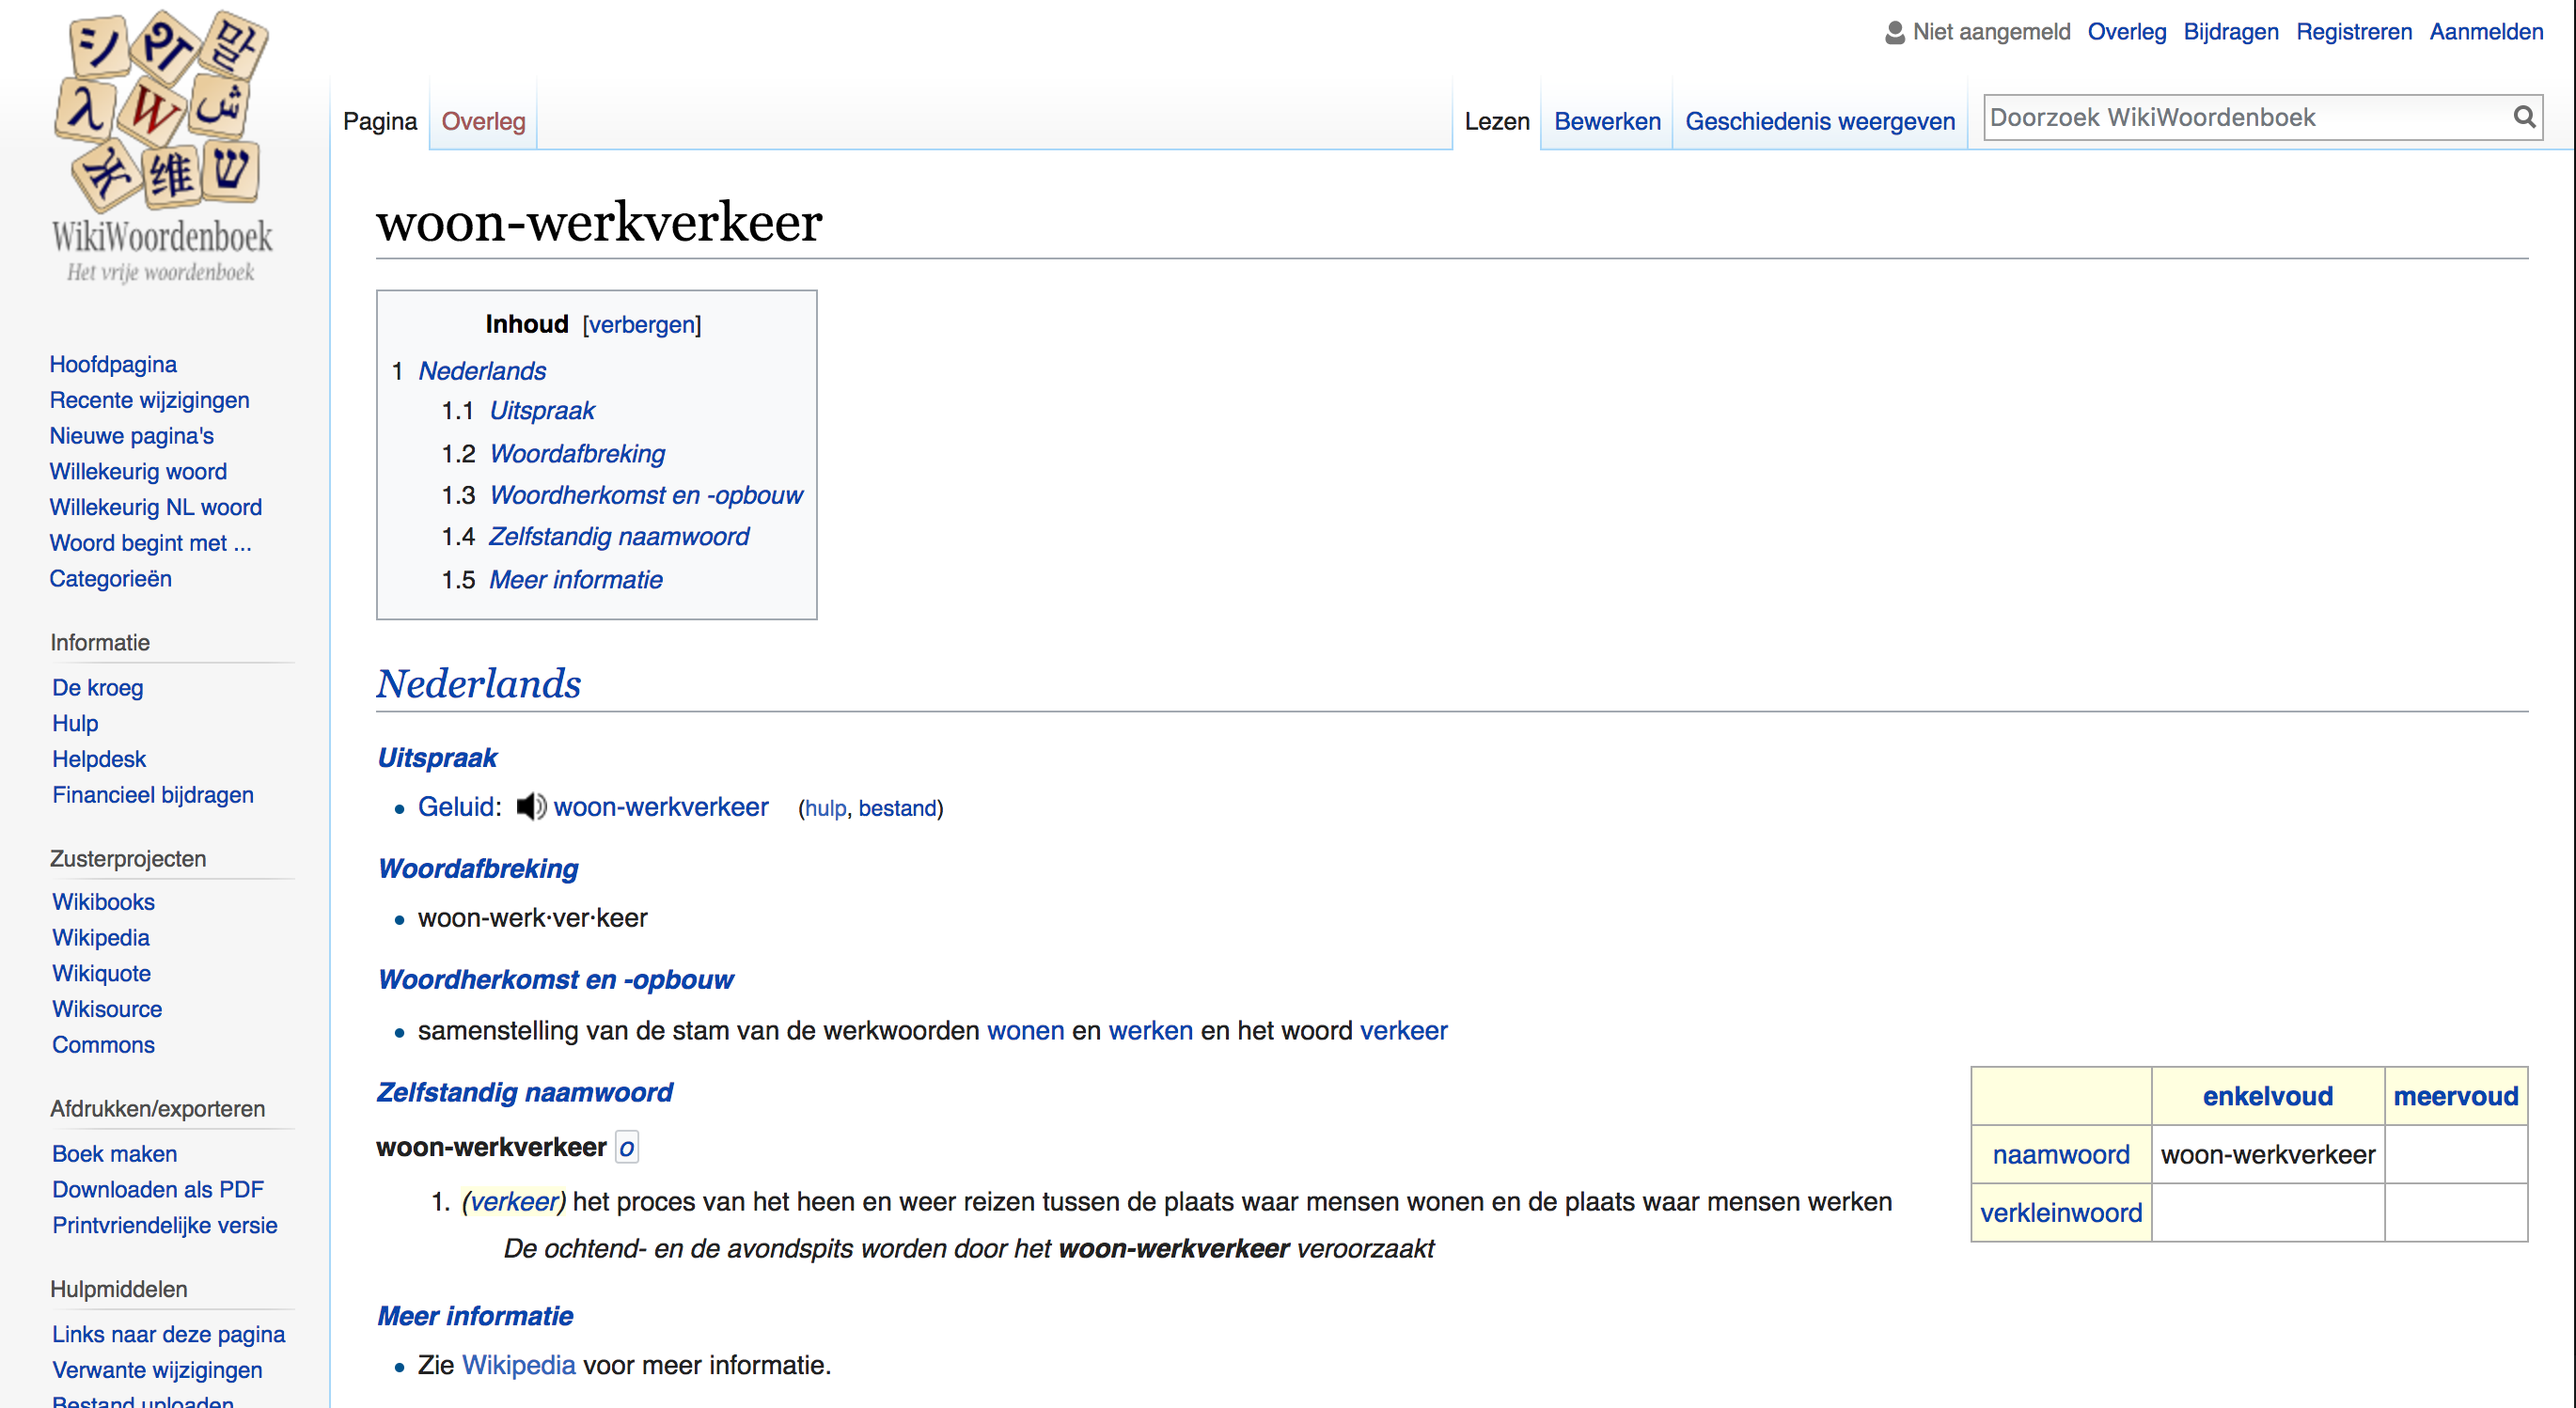
\includegraphics[width=0.8\textwidth]{useless_page}
\caption{Example of an undesired result obtained with Google Custom Search}
\label{fig:useless_page}
\end{figure}

Finally, we decided to provide our clients with a "labelling interface". This way, we have total control of the documents that are added to the data set. The documents are labelled by experts in the field of the built environment so we may assume these documents will represent the labelled categories well. The labelling interface provides the user with a document from the set of collected documents. It allows the user to label these documents with zero or more categories, after which the document is saved to the training set(s) corresponding to correct categories. If no category is selected, the document is discarded from the training set. 

\begin{figure}[h]
\centering
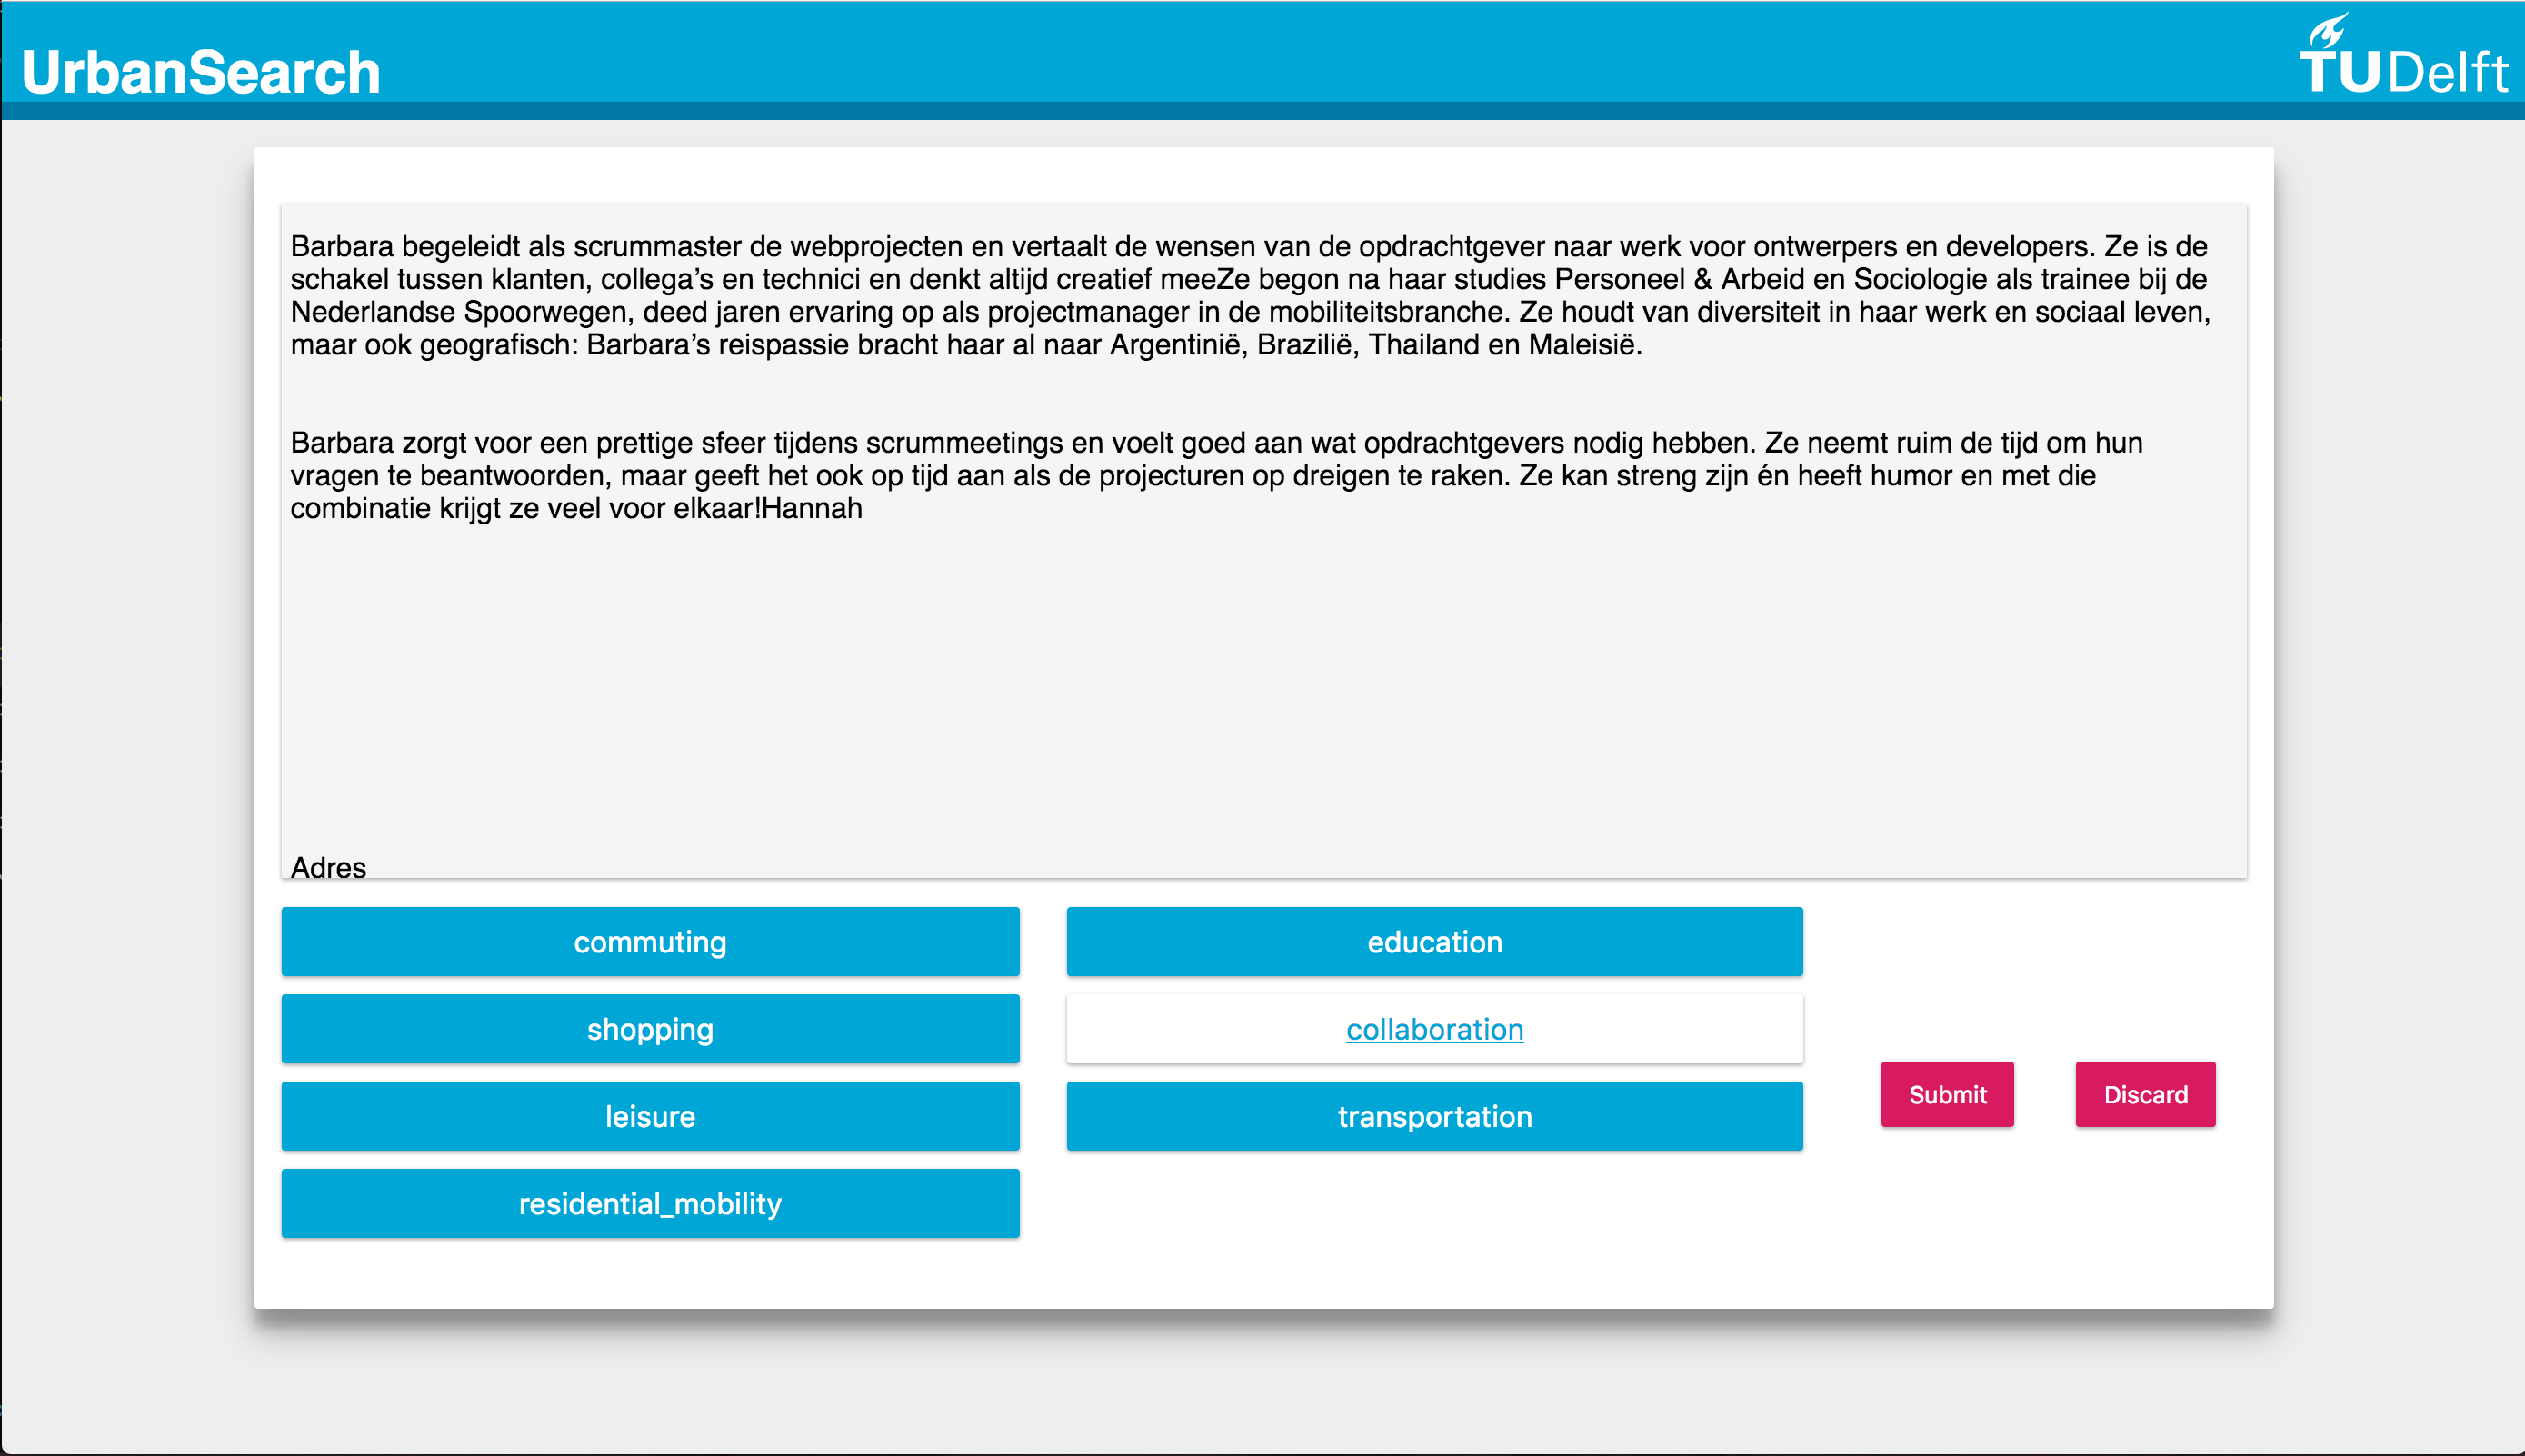
\includegraphics[width=0.8\textwidth]{labelling_interface}
\caption{Labelling interface}
\label{fig:labelling_interface}
\end{figure}

\subsection{Modelling}
When considering classification, there are a plethora of algorithms available. When choosing the right algorithm for a problem, several factors should be taken into account\cite{MLCheatSheet}. These are:
    \begin{description}
        \item[\textbf{Accuracy}] How well the algorithm separates the documents.
        \item[\textbf{Training Time}] How long it takes to train the algorithm.
        \item[\textbf{Linearity}] Some problems can be solved by splitting classes using a straight line. For other problems this approach is not feasible.
        \item[\textbf{Number of Parameters}] Adjustable parameters increase the flexibility of the algorithms. This is a trade-off between training time and accuracy.
        \item[\textbf{Number of Features}] A large number of features can make some algorithms slow. Extracting features from text-data often results in a huge feature set (65000+ in our case).
        \item[\textbf{Special Cases}] Some learning algorithms make particular assumptions about the data or the results (eg. rank prediction, count prediction). This way we can increase desirable properties like accuracy of the prediction or improved training times. 
    \end{description}

Keeping all these properties in mind we construct a setup that fits our purposes best.
Below we have stated our approach of how we reached the setup we think is best suited for our goals.

%Lots of machine learning algorithms make use of linearity. Linear classification algorithms assume that classes can be separated by a straight line (or its higher-dimensional analog).  These include logistic regression and support vector machines (as implemented in Azure Machine Learning). Linear regression algorithms assume that data trends follow a straight line. These assumptions aren't bad for some problems, but on others they bring accuracy down. Despite their dangers, linear algorithms are very popular as a first line of attack. They tend to be algorithmically simple and fast to train.

\begin{description}
\item[\textbf{Features}] 
To get a useful set of inputs (features) for our system we need to decide what describes the properties of our documents best. Since we are dealing with text-documents a natural choice for these inputs are the words contained in these documents. 
The words alone do not provide us a very useful input to the system. That is why we use TF-IDF to give the words that we encountered a weight. TF-IDF (Term Frequency over Inverse Document Frequency) gives words a weight based on their frequency in a document and on the frequency of the word in the complete document set. This way words that are rare in the complete document set but occur often in a document are assigned a high weight. Words that occur in many documents in the complete document set get awarded a low weight\cite{ramos_tfidf}.
Using TF-IDF our features become words with weights associated to them.

\item[\textbf{Dimensionality Reduction}]
Since we are working with text documents and our features are words with TF-IDF weights we can assume that our feature set will be very large (65000+). The total number of features determines how fast we can train our model and has implications regarding over-fitting \cite{ml_text}. To reduce the number of features we considered different techniques from \cite{ml_text}. Since we have no time to test all the techniques, we decided to select the top ten percent of our features (based on the TF-IDF weights). In \cite{yang1997} it is stated that a dimensionality reduction with a factor ten using this approach does not lead to a loss in accuracy when classifying text documents. To provide an easy way to add different types of dimensionality reduction techniques later, we will keep the code for defining new Scikit pipelines, which are the basic construct used for creating our classifiers, easily extendable.

\item[\textbf{Classification}]
Even after applying dimensionality reduction which we discussed in the previous section, we are left with a lot of features (6500+). Thus, we need an algorithm that works well with a feature rich problem. From \cite{MLCheatSheet} we know Support Vector Machines(SVM) is a algorithm that works well with feature rich problems. Also \cite{ml_text} claims SVM is one of the best techniques when considering text classification. This combined with the fact that Scikit offers an easy to use implementation of SVM has lead us to use SVM as our classification algorithm. The concept of a SVM is that of a hyper-plane that divides two distinct sets, while trying to maximise the margin between these sets \cite{tong2001support}.
\end{description}

\subsection{Remarks}
Scikit offers a lot of useful features to optimise the classifier. For example, using Scikit pipelines combining a classifier with several transforms (eg. dimensionality reduction transforms) is an relatively easy task. Since we unfortunately do not have the time to benchmark the results of different types of classifiers and to play around with the different optimisation options, we plan on implementing our code in such a way that extending the code to use these optimising functionality and different pipelines will be really easy.
